\documentclass{article}

% if you need to pass options to natbib, use, e.g.:
%     \PassOptionsToPackage{numbers, compress}{natbib}
% before loading neurips_2021

% ready for submission
\usepackage[preprint]{neurips_2021}

% to compile a preprint version, e.g., for submission to arXiv, add add the
% [preprint] option:
%     \usepackage[preprint]{neurips_2021}

% to compile a camera-ready version, add the [final] option, e.g.:
%     \usepackage[final]{neurips_2021}

% to avoid loading the natbib package, add option nonatbib:
%    \usepackage[nonatbib]{neurips_2021}

\usepackage[utf8]{inputenc} % allow utf-8 input
\usepackage[T1]{fontenc}    % use 8-bit T1 fonts
\usepackage{hyperref}       % hyperlinks
\usepackage{url}            % simple URL typesetting
\usepackage{booktabs}       % professional-quality tables
\usepackage{amsfonts}       % blackboard math symbols
\usepackage{nicefrac}       % compact symbols for 1/2, etc.
\usepackage{microtype}      % microtypography
\usepackage{xcolor}         % colors

% proper quoting
\usepackage{csquotes} 

\usepackage{graphicx}



\title{Effects of Conventional and Renewable Electricity Generation on Spot Market Prices in Germany and Luxembourg}

% The \author macro works with any number of authors. There are two commands
% used to separate the names and addresses of multiple authors: \And and \AND.
%
% Using \And between authors leaves it to LaTeX to determine where to break the
% lines. Using \AND forces a line break at that point. So, if LaTeX puts 3 of 4
% authors names on the first line, and the last on the second line, try using
% \AND instead of \And before the third author name.

\author{%
Ismail Kisa\\
% Matrikelnummer \\
\texttt{ismail.kisa@student.uni-tuebingen.de}\\
\And Gereon Recht\\
% Matrikelnummer \\
\texttt{gereon.recht@student.uni-tuebingen.de} \\
  %David S.~Hippocampus\thanks{Use footnote for providing further information
   % about author (webpage, alternative address)---\emph{not} for acknowledging
   % funding agencies.} \\
  %Department of Computer Science\\
  %Cranberry-Lemon University\\
  %Pittsburgh, PA 15213 \\
  %\texttt{hippo@cs.cranberry-lemon.edu} \\
  % examples of more authors
  % \And
  % Coauthor \\
  % Affiliation \\
  % Address \\
  % \texttt{email} \\
  % \AND
  % Coauthor \\
  % Affiliation \\
  % Address \\
  % \texttt{email} \\
  % \And
  % Coauthor \\
  % Affiliation \\
  % Address \\
  % \texttt{email} \\
  % \And
  % Coauthor \\
  % Affiliation \\
  % Address \\
  % \texttt{email} \\
}

\begin{document}

\maketitle

\begin{abstract}
\begin{itemize}
    \item Increasing renewable generation in Germany $->$ EEG (Erneurbare Energien Gesetz) responsible for that
    \item This paper analyses the effect of renewabele/conventional generation on the spot market price
    \item Analyzed interval from 2019 - 2021
    \item Describe data briefly
    \item We use regression analysis
    \item Mention result: negative correlation of renewable generation and price $->$ merit-order
\end{itemize}


\end{abstract}

\section{Introduction}

\begin{itemize}
    \item explain why negative prices can occur
\end{itemize}

In today's liberalized electricity markets, electricity is traded in megawatt hours (MWh), where one MWh denotes the generation of one MW over the duration of one hour \citep{markets_for_electrical_energy}.
Thus, electricity markets have fixed time intervals serving as trading periods.
Trading within shorter time intervals better reflects the physical conditions of the energy system.
But this is not desired e.g.\ by agents who run base load generators, which constantly produce to meet the minimum demand, as they rather want a fixed price and quantity over a larger time interval in order to reduce their risks.
Hence, there are different electricity markets which trade over different time intervals.
On forward markets, electricity is traded well before its consumption in larger amounts.
Spot markets trade in the shortest time intervals, e.g.\ quarter-hourly, and are important for balancing demand and generation, which have to be equal at all times to ensure the stability of the system.
Prices on spot markets are based on the bids and offers of the agents and are set by the market operator, who manages the market.
To meet the demand, the market operator prioritizes cheaper generators.
This leads to the \enquote{merit order}, an ordering of generators by their marginal costs, i.e.\ the cost of supplying one additional marginal unit of power.
The most expensive generator needed to meet the demand sets the price.
As renewable energy sources like wind and photovoltaic (PV) have near-zero marginal costs, they enter at the bottom of the merit-order and thus depress market prices when they generate a substantial amount of electricity.
This is called the \enquote{merit-order effect}.
% TODO: find citation for merit-order - somehow not in that book??

Electricity generation can be divided into two categories: conventional and renewable. Conventional power generation refers to those power plants that require finite, fossil energy resources. These include gas, coal or oil but also nuclear power plants. On the otherside, renwable power generation uses energy sources that are continously renewed and are available unlimited. Examples are hydropower, photovoltaic, wind or biomass. Our data contains, besides the mentioned power plants, "other renewables" and "other conventionals". "Other renewables" include for example geothermal energy or landfill gas. "Other conventionals" incude trash or mineral oil. Those power plants have a small electricity generation and are merged. The most significant energies are wind and solar for renewable, and brown coal and nuclear for conventional. 

\section{Data}
We use time series data from the years 2019 to 2021 of hourly electricity generation separated by technology type and quarter-hourly intraday spot market prices, both for the bidding zone comprised of Germany and Luxembourg \citep{smard}.
Bidding zones are areas which have the same electricity price.
We transform the spot market prices to hourly intervals by taking the mean value for each hour in order to relate them to the electricity generation data.
The data represents the net electricity generation fed into the general supply electricity network wihtout the own needs of the power plants.

SMARD obtains most of the data directly from the transparency platform European Transmission System Operators (ENTSO-O). 
Each european transmission system operator (TSO) as well as the power market exchange are obliged to report and publish their data for their respective bidding zone, according to the Electricity Trancparency Regulation (Regulation (EU) No. 543/2013), at the ENTSO-O at the latest in one hour.
Only data verified by the federal network agency is published on SMARD \cite{smard_usermanual}.

Despite Pumped-Storage hydro uses hydropower to generate electricity, it is classified as a conventional source in the user manual of SMARD \cite{smard_usermanual}. Since Pumped-Storage hydro needs a special treatment, we will analyze it seperately.  

TODO: Understand user manual page 38. So far I understood that some values are estimates.
\begin{figure}[h]
    \centering
    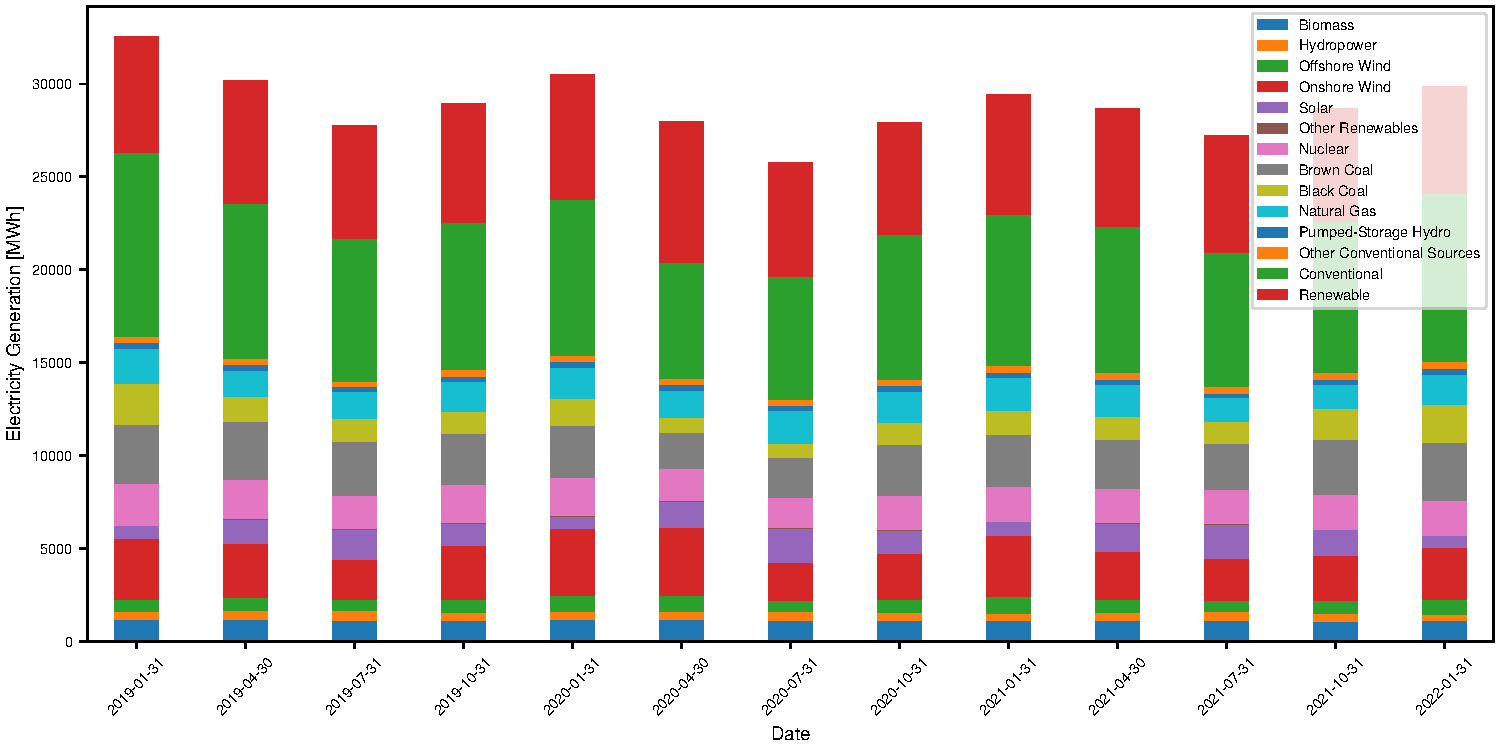
\includegraphics[width=0.8\columnwidth]{doc/fig/quarterly_technology_mix.pdf}
    \caption{Caption}
    \label{fig:quarterly_mix}
\end{figure}


\begin{itemize}
    \item Mention that the price has increased a lot since 2019, while the percentage of renewable is same?
    \\
    \item Informations from \textit{https://www.smard.de/page/home/wiki-article/446/636, https://www.smard.de/page/home/wiki-article/518/562}
    \item Introduce data by showing exemplary day, maybe one where renewables depress prices
\end{itemize}

\section{Methods}

\section{Results}

\begin{itemize}
    \item Figure \ref{fig:ren_vs_con_regression} shows the opposite effects of renewable and conventional electricity generation on the prices.
    \item Data and analysis can be found on Github \citep{github_repo}.
\end{itemize}

\begin{figure}
    \centering
    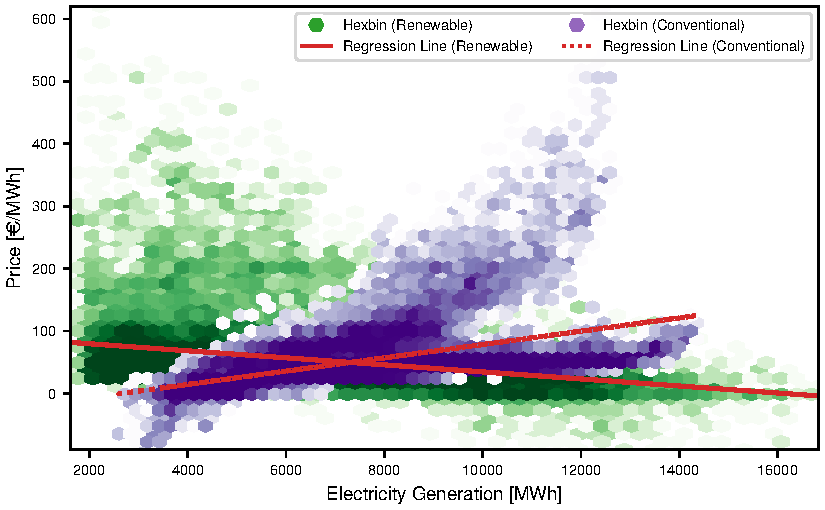
\includegraphics[width=0.7\columnwidth]{doc/fig/ren_vs_con_regression.pdf}
    \caption{Caption}
    \label{fig:ren_vs_con_regression}
\end{figure}

\begin{figure}
    \centering
    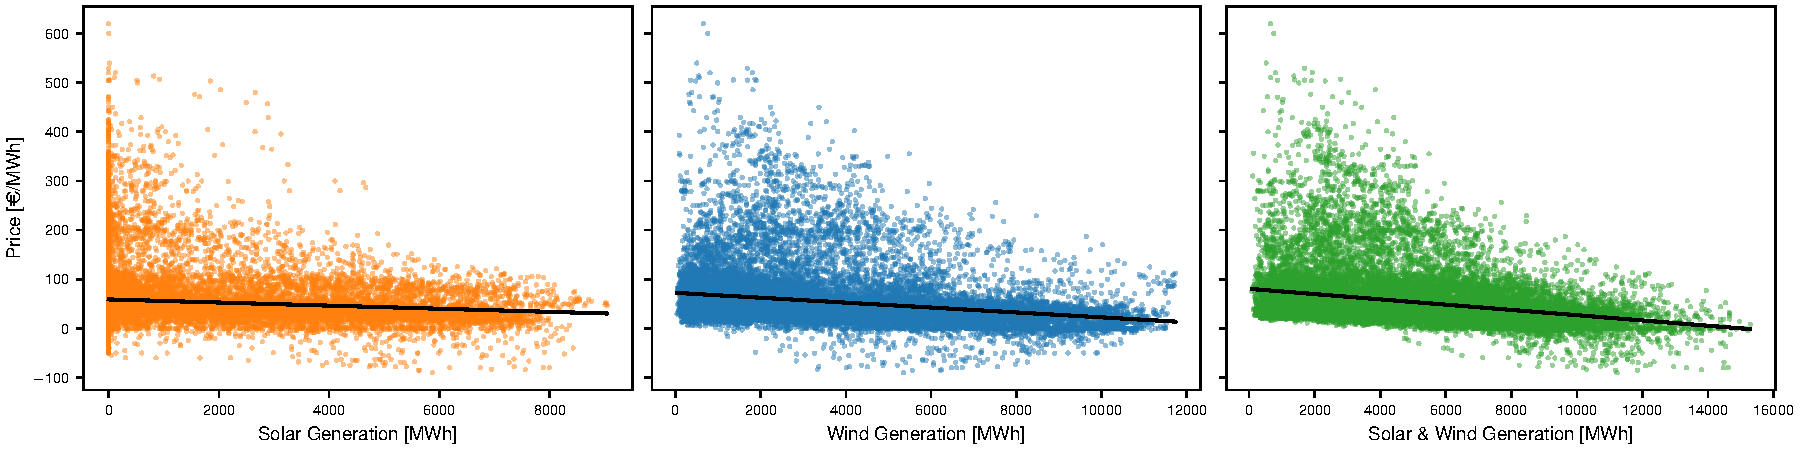
\includegraphics[width=\columnwidth]{doc/fig/solar_wind_regression.pdf}
    \caption{Caption}
    \label{fig:solar_wind_regression}
\end{figure}

\begin{figure}
    \centering
    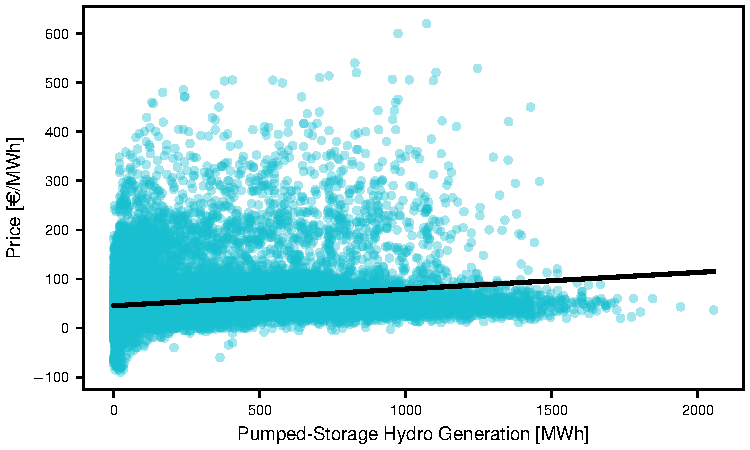
\includegraphics[width=0.7\columnwidth]{doc/fig/pumped_hydro_regression.pdf}
    \caption{Caption}
    \label{fig:pumped_hydro_regression}
\end{figure}

\section{Conclusion}

\bibliographystyle{plainnat}
\bibliography{literature}
\end{document}
